\section{Fremgangsmetode}

Da den integrerede kreds, BQ76920, nærmest var valgt på forhånd, var næste skridt at finde en microcontroller der kunne styre kredsen. Derefter blev softwaren udviklet, og de tilhørende komponenter dimensioneret. 
\klp{Hvorfor var den valgt på forhånd? Hvad kan den?}

\sbf{kom ind under spændingsnet 20mah vs 200mah}

\section{Valg af microcontroller}\label{afs:valg_af_uc}
Der blev besluttet at bruge microcontrolleren LPC804 til denne BMS. Den blev valgt af flere årsager:
\begin{itemize}
	\item Lavt strømforbrug i deep sleep.
	\item ADC i 12-bits opløsning.
	\item De ønskede interfaces er tilgængelige. ($I^2C$, $UART$)
	\item Microcontrolleren er NXP's billigere serie. 
	\item Fås i både relativt små pakker samt store pakker.
	\item Evaluationboard er tilgængeligt.
\end{itemize}

Evaluationsboardet ved navn UM40001UL bliver brugt til udvikling af software. Dette board har onboard CMSIS-DAP som er en debugger, således det ikke er nødvendigt med en ekstern debugger. 

\section{Batteriovervågningskreds}
Den integrerede kreds der er valgt klarer nærmest alle opgaver. Den står for overvågning af cellespændinger, balancering, styring af MOSFET's (charge og discharge), mulighed for ekstra temperaturstyring samt coloumb counting (strømmåling). \\

\begin{figure}[h]
	\centering
	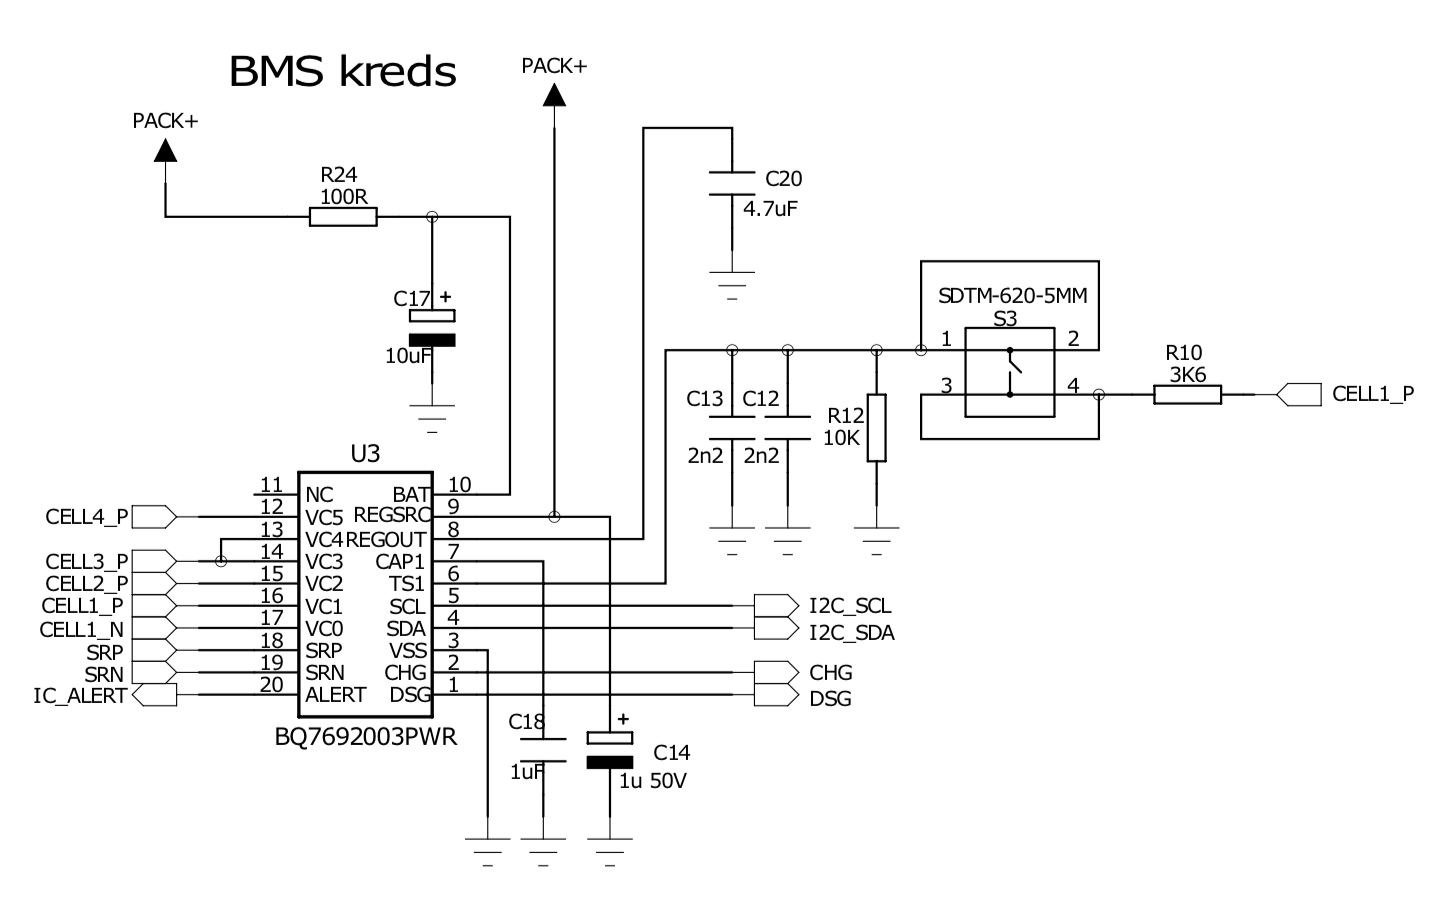
\includegraphics[width=15cm]{billeder/bms_ic_sch.png}
	\caption{Schematics for balanceringskredsen}
	\label{fig:temp_sensor}
\end{figure}

Da kredsen fungerer vha. kommunikation over I2C, sættes den først og fremmest til I2C bus'en. SDA er datalinjen og SCL er clock linjen. \\

\sbf{Andet navn for balanceringskreds}
\sbf{Kom in under alert ben og deres transistorer }
\sbf{Kom ind under FET's}

\section{Temperatursensor}
Som endnu en sikkerhedsforanstaltning bruges en temperatursensor til at overvåge temperaturen i batteripakken. Her blev der besluttet at bruge en I2C temperatursensor, da opsætning ville være nemt siden I2C allerede skulle benyttes. Den specifikke del hedder LM75BIM-3/NOPB. Denne model blev valgt da den var tilgængelig på evaluation-boardet af microcontrolleren som blev brugt under udvikling. Derfor kunne udviklingen af software ske før hardware delen var helt færdig, og dermed fremskynde processen en smule. \\

\subsection{Tilslutning af sensor}
Siden sensoren benytter I2C, er den relativt nemt at sætte til i hardware. SCL og SDA sættes til I2C bus'en på microcontrolleren, og OS benet sættes til et vilkårligt GPIO ben på microcontrolleren. 
\sbf{Andet ord for "sætte til"?}

\begin{figure}[h]
	\centering
	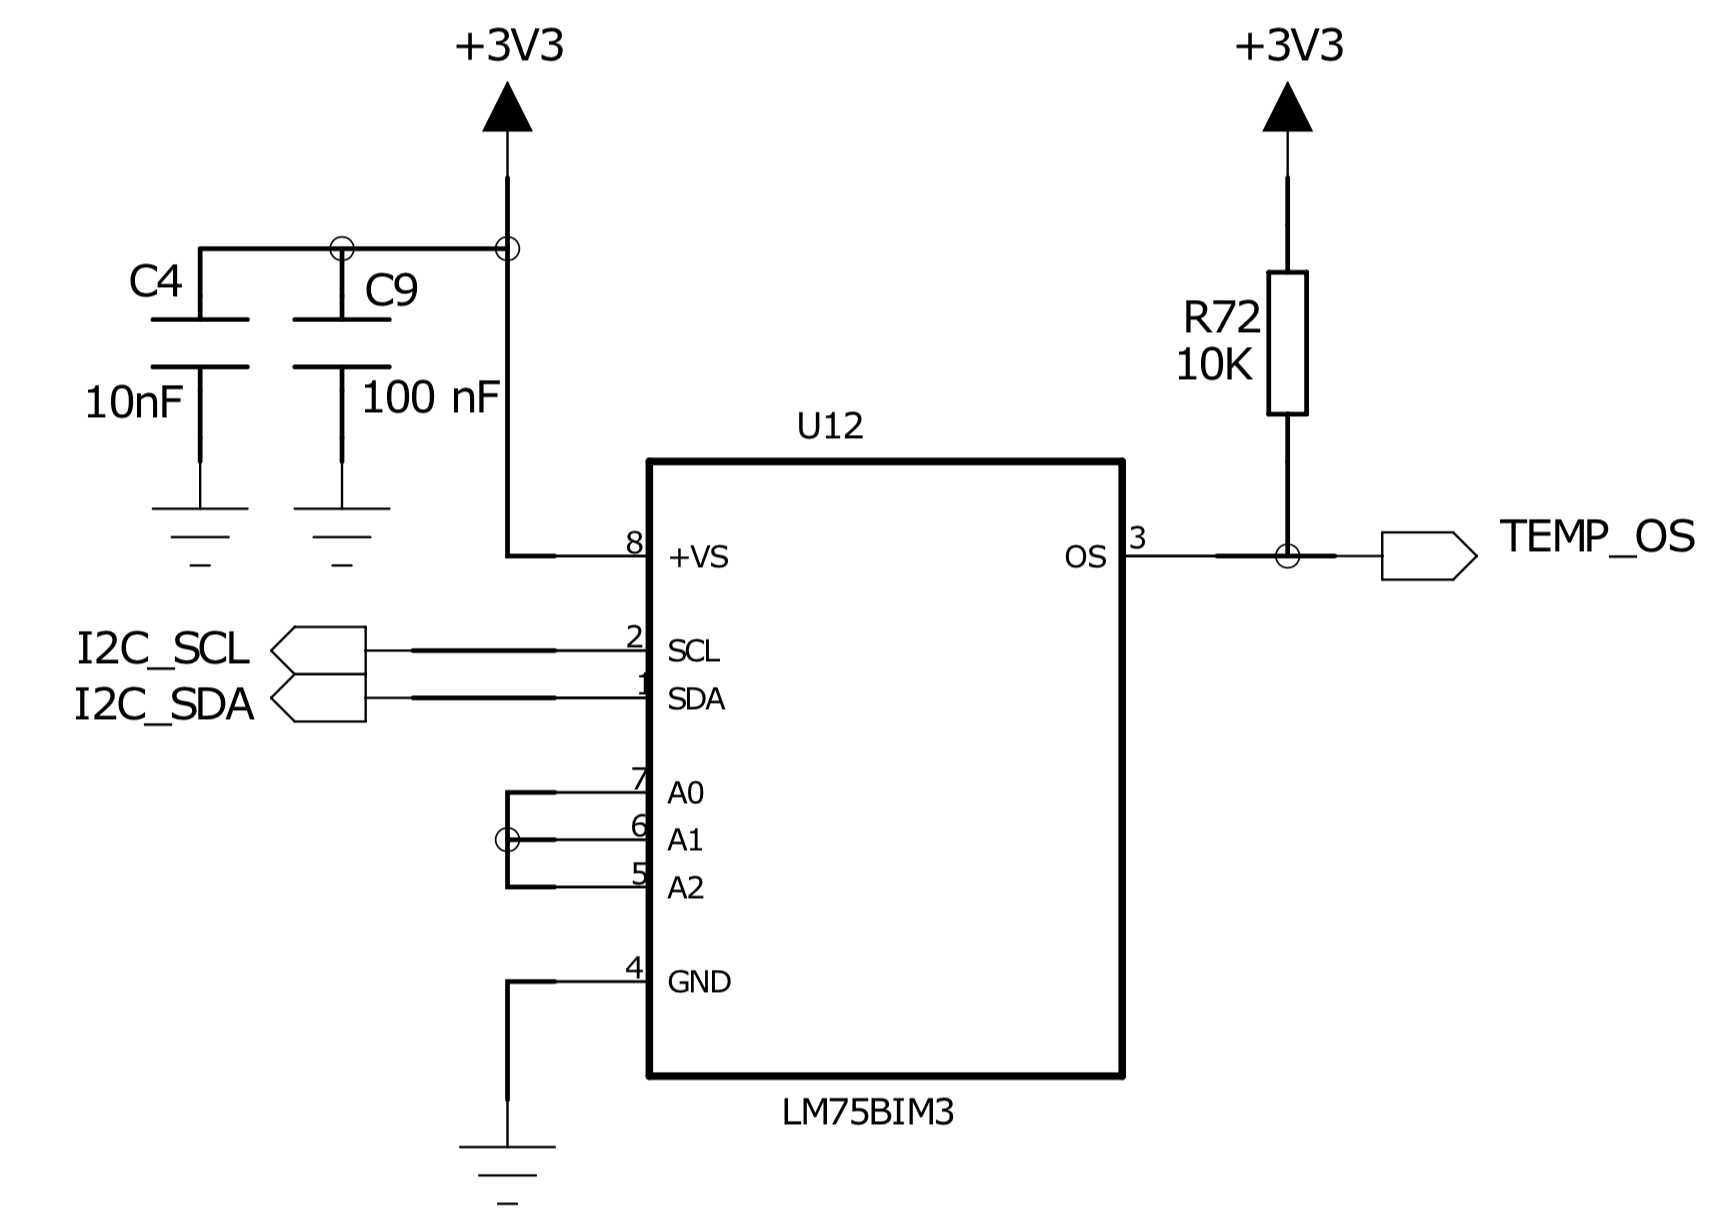
\includegraphics[width=11cm]{billeder/temp_sensor_sch.png}
	\caption{Schematics for temperatursensor}
	\label{fig:temp_sensor}
\end{figure}

Dette ben (OS) er til eventuelle status meddelelser fra sensoren. Bliver ikke brugt i dette system, men er stadig tilføjet for eventuelt fremtidigt brug. Implementering af sensoren i software diskuteres i kapitel \ref{kap:softwareudvikling}.

\sbf{Cellebalancering og strømmåling}